\documentclass[border=0.2cm]{standalone}
\usepackage{tikz}
\usetikzlibrary{calc}
\begin{document}
\pagestyle{empty}
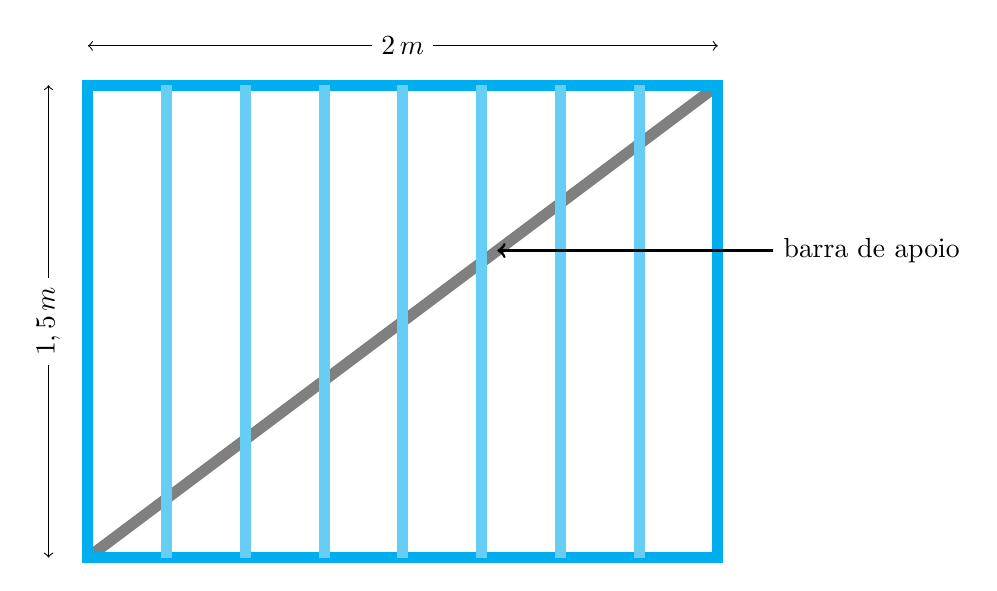
\begin{tikzpicture}


 \draw[line width=4pt,gray] (-4,-3) -- (4,3);
 \draw[line width=4pt,cyan] (-4,-3) rectangle (4,3);
 \foreach \x in {-3,...,3} {
 \draw[line width=4pt,cyan!60] (\x,-3) -- (\x,3);
 }
 \draw[<->] (-4,3.5) -- (4,3.5) node[midway,fill=white] {$2\,m$};
 \draw[<->] (-4.5,-3) -- (-4.5,3) node[midway,fill=white,rotate=90] {$1,5\,m$};
 
 \draw[line width=1pt, <-] ($(0,0)!0.3!(4,3)$) -- +(3.5,0) node[right] {barra de apoio};

\end{tikzpicture}

\end{document}